\documentclass{article}
\usepackage{style}
\begin{document}
\maketitle
\tableofcontents
\section{Introducción}
En esta práctica se implementaron los algoritmos:
\begin{itemize}
	\item Un punto de cruza.\\
	Fue propuesto por Holland, fue el algoritmo de cruza más popular, pero hoy en día no lo es debido a sus inconvenientes.
	\item Dos puntos de cruza.\\
	Propuesto por DeJong, los dos puntos minimizan los efectos destructivos del algoritmo y se considera mejor que el un solo punto.
	\item Uniforme.\\
	Propuesto por Ackley, se genera una máscara de bits, la cual suele usarse con $P_c = 0.5$, para evitar los resultados destructivos. 
	\item Cruza Acentuada. \\
	Propuesto por Schaffer y Morishima, parecido al uniforme se seleccionan los bloques de construcción ``buenos'', los cuales son copiados a los hijos.
\end{itemize}
\newpage
\section{Contenido}
\subsection{Un punto de cruza}
\begin{figure}[h!]
	\centering
	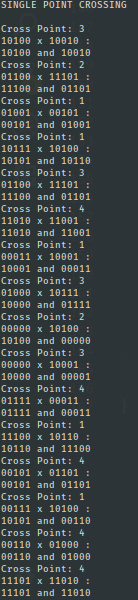
\includegraphics[scale=.3]{single}
\end{figure}
\newpage
\subsection{Dos puntos de cruza}
\begin{figure}[h!]
	\centering
	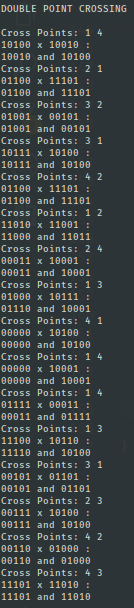
\includegraphics[scale=.3]{double}
\end{figure}
\newpage
\subsection{Uniforme}
\begin{figure}[h!]
	\centering
	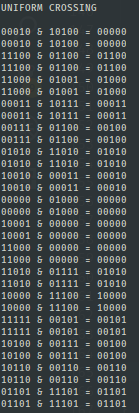
\includegraphics[scale=.3]{uniform}
\end{figure}
\newpage
\subsection{Acentuada}
\begin{figure}[h!]
	\centering
	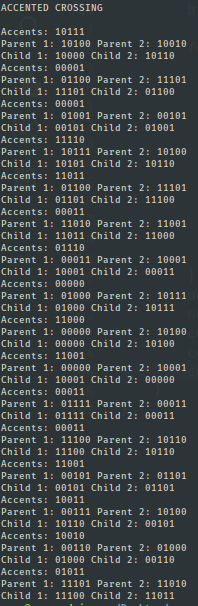
\includegraphics[scale=.3]{accented}
\end{figure}
\section{Conclusión}
En esta práctica se pudieron ver las diferencias de algunos de los algoritmos más populares de cruza, se implementaron y se analizaron.
\end{document}